\subsection{Simple Experiments}
\label{sec:appendix_simple_experiments}

\subsubsection{k--Summation Problem Definition}
\label{sec:a_se_prob_def}

Here we look at a synthetic, simple task in order to investigate the behavior of softmax and sigmoid attention activations.  The problem chosen is to minimize the MSE loss of a $\mathbb{R}^{n} \rightarrow \mathbb{R}$ target function.  In the first half of each input are samples from a $\mathcal{N}(0,1)$ distribution, and the second half is a $k$-hot binary vector indicating which values in the first half to sum.  

The results presented here are for the $n=40$ problem with various values for $k$.  Where a transformer is used, the transformer is a single layer to aid visualization.  In all cases (unless noted otherwise), the optimizer is Adam with a constant learning rate of 0.001, and the training data is continuously generated to preclude over-fitting.

A few examples for $n=10$ (not drawn from $\mathcal{N}(0,1)$) are shown below.  Inputs in the second half of the input are show in {\color{orange} orange} only as a visual aid.

\begin{table}[h]
    \centering
    \begin{tabular}{c}
        \texttt{1 2 3 4 5 {\color{orange} 0 0 0 0 1 }$\rightarrow$ 5} \\
        \texttt{1 2 3 4 5 {\color{orange} 1 0 0 0 1 }$\rightarrow$ 6} \\
        \texttt{8 1 2 0 5 {\color{orange} 0 1 1 1 0 }$\rightarrow$ 3} \\
        \texttt{2 0 2 2 2 {\color{orange} 1 1 0 1 0 }$\rightarrow$ 4} \\
    \end{tabular}
    \label{tab:k_sum_examples}
\end{table}

\subsubsection{Comparison to Softmax}
\label{sec:a_se_compare}

In \Cref{fig:final_loss_k_summation}, we see the performance of three architectures on the $k$-summation problem as $k$ increases.  The sigmoid activated transformer has similar scaling to the softmax activation.

\begin{figure}[h]
    \centering
    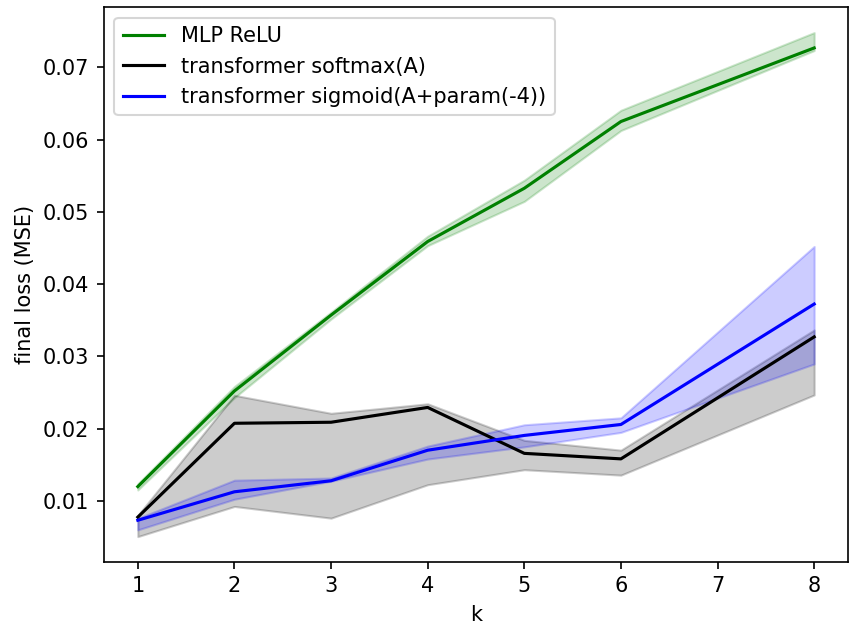
\includegraphics[width=0.6\textwidth]{figures/final_loss_vs_k_summation.png}
    \caption{Final loss is shown after training convergence as k-summation problem complexity increases. The ReLU MLP has two hidden layers (900, 300) for 307k parameters, while the transformer has an embedding dimension of 120, 8 heads, and an MLP ratio of 4, giving 187k parameters. The $\sigmoidattn$ is applied after a learned offset initialized to -4, \texttt{A+param(-4)}.}
    \label{fig:final_loss_k_summation}
\end{figure}

\subsubsection{Attention Evolution}
\label{sec:a_se_evo}

In \Cref{fig:attn_evolve,fig:attn_metric_evolve}, forty samples are used to monitor the single head, single layer post-activation attention matrix as training progresses.   In \Cref{fig:attn_evolve}, the distribution of values is visualized over time; note the sigmoid attention is more variable but reaches comparable values at convergence.  The main difference at convergence is that the sigmoid has fewer high magnitude values than softmax indicating a more distributed attention.  

\begin{figure}[h]
  \centering
  \begin{minipage}[b]{0.45\textwidth}
    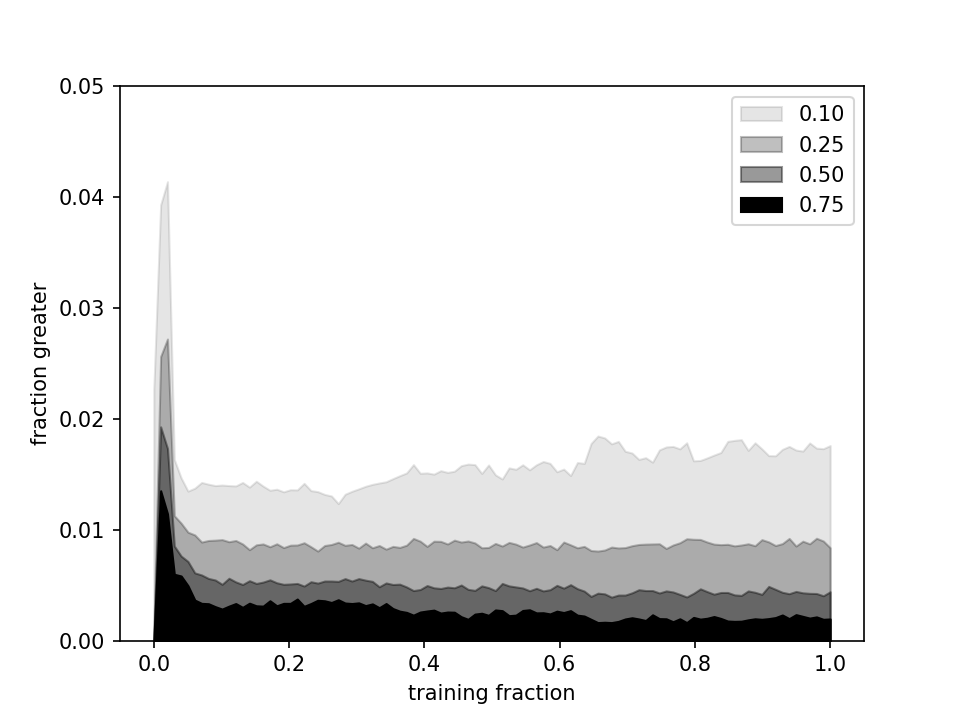
\includegraphics[width=\textwidth]{figures/trans_softmax_attn_fraction.png}
    \captionsetup{labelformat=empty}
    \caption{Softmax}
    \addtocounter{figure}{-1}
  \end{minipage}
  \hfill
  \begin{minipage}[b]{0.45\textwidth}
    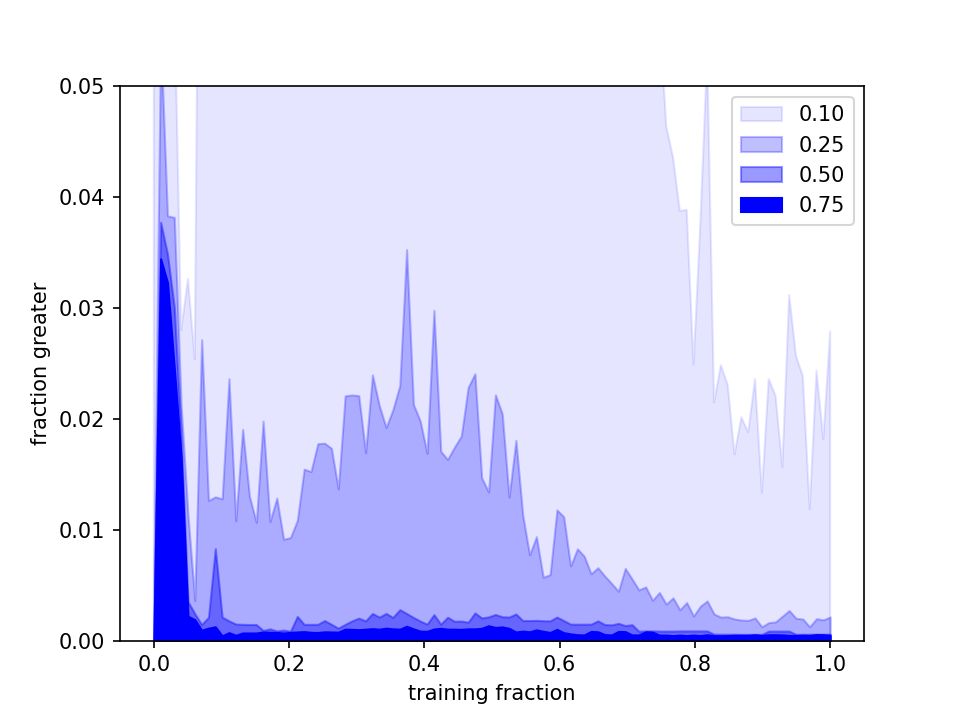
\includegraphics[width=\textwidth]{figures/trans_sigmoid,-4,False_attn_fraction.png}
    \captionsetup{labelformat=empty}
    \caption{Sigmoid}
    \addtocounter{figure}{-1}
  \end{minipage}
  \caption{The post-activation attention evolves during training on the $k=1, n=40$ summation problem.  The model has one head to simplify the visualization. Forty repeated test samples are used.}
  \label{fig:attn_evolve}
\end{figure}

In \Cref{fig:attn_metric_evolve}, metrics on the post-activation attention matrices are used and show comparable behavior in the first half of training.  
In the second half of training, the $\sigmoidattn$ can be seen to reduce in norm and in sparsity. (see following discussion of \Cref{fig:attn_by_sample} for further insights).

\begin{figure}[h]
  \centering
  \begin{minipage}[b]{0.45\textwidth}
    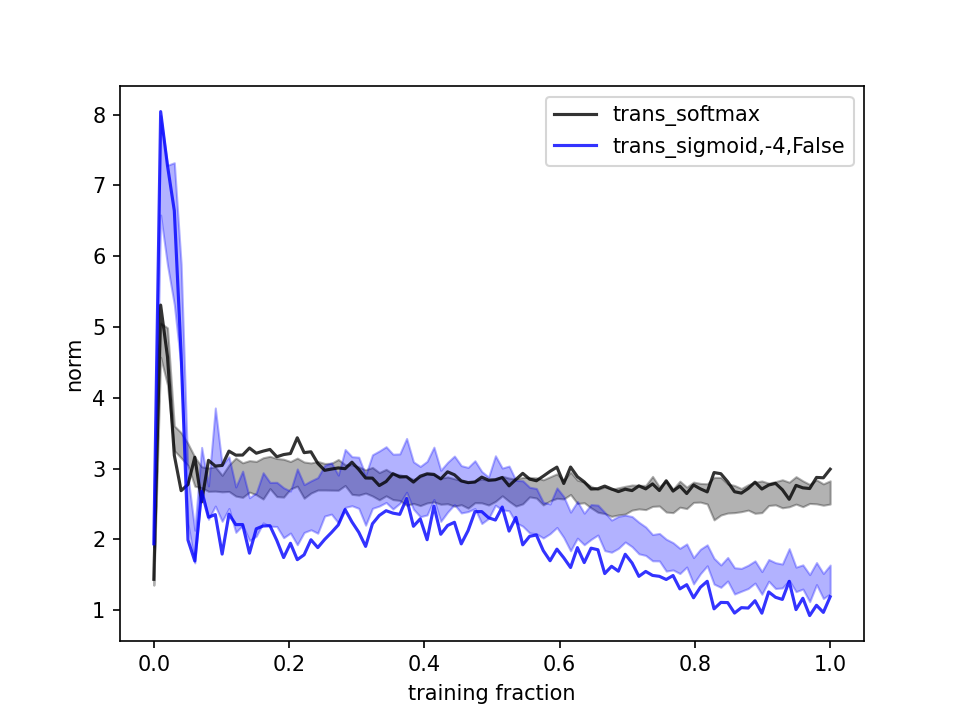
\includegraphics[width=\textwidth]{figures/norm_training_1_head.png}
    \captionsetup{labelformat=empty}
    \caption{Norm}
    \addtocounter{figure}{-1}
  \end{minipage}
  \hfill
  \begin{minipage}[b]{0.45\textwidth}
    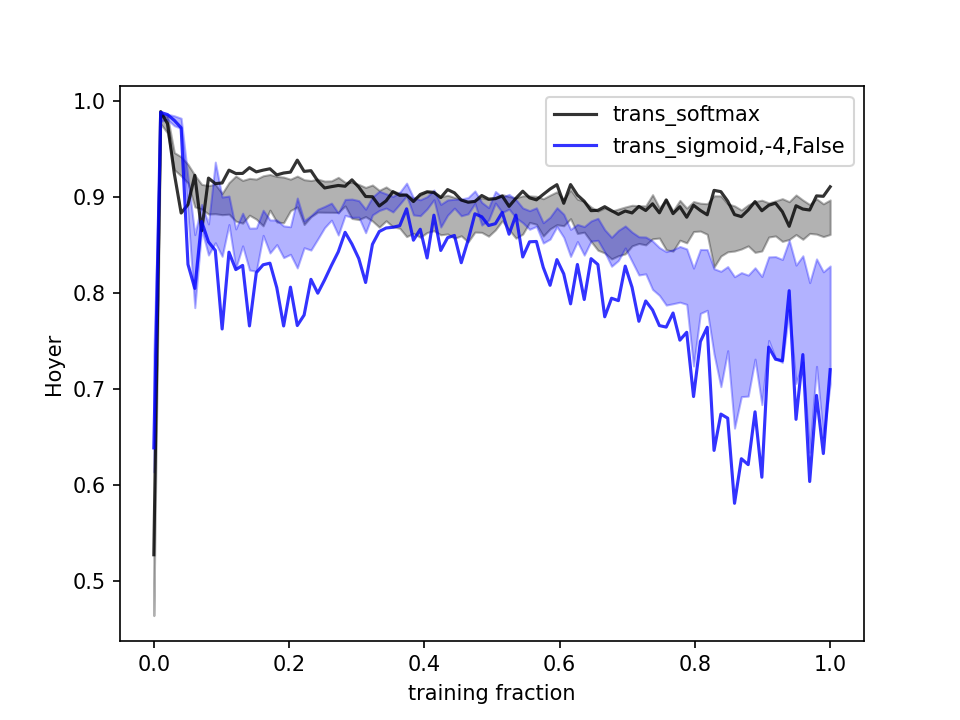
\includegraphics[width=\textwidth]{figures/hoyer_training_1_head.png}
    \captionsetup{labelformat=empty}
    \caption{Hoyer Sparsity}
    \addtocounter{figure}{-1}
  \end{minipage}
  \caption{ Metrics on the post-activation attention evolve during training on the $k=1, n=40$ summation problem.  The model has one head to simplify the visualization. Quartiles and mean from 40 repeated test samples are shown. On the right, the Hoyer Sparsity~\citep{hurley2009comparing} is used to measure the change in sparsity as training progresses: $\text{Hoyer} := \left(\sqrt{n}-\frac{\sum_j c_j}{\sqrt{\sum_j c_j^2}}\right)(\sqrt{n}-1)^{-1}$.
  }
  \label{fig:attn_metric_evolve}
\end{figure}

In \Cref{fig:attn_by_sample}, we see post-activation attention values for eight samples at training progresses.  The most notable difference between the activations is, that by the end of training, the $\sigmoidattn$ is less sparse in the $\mathcal{N}(0,1)$ self-attention in the upper-left quadrant.  We can see that softmax tends to produce sparser values (as it is designed to) while sigmoid controls the magnitude and location of peak attention independently, leading to a less sparse attention at the end of training.

\begin{figure}[h]
    \centering
    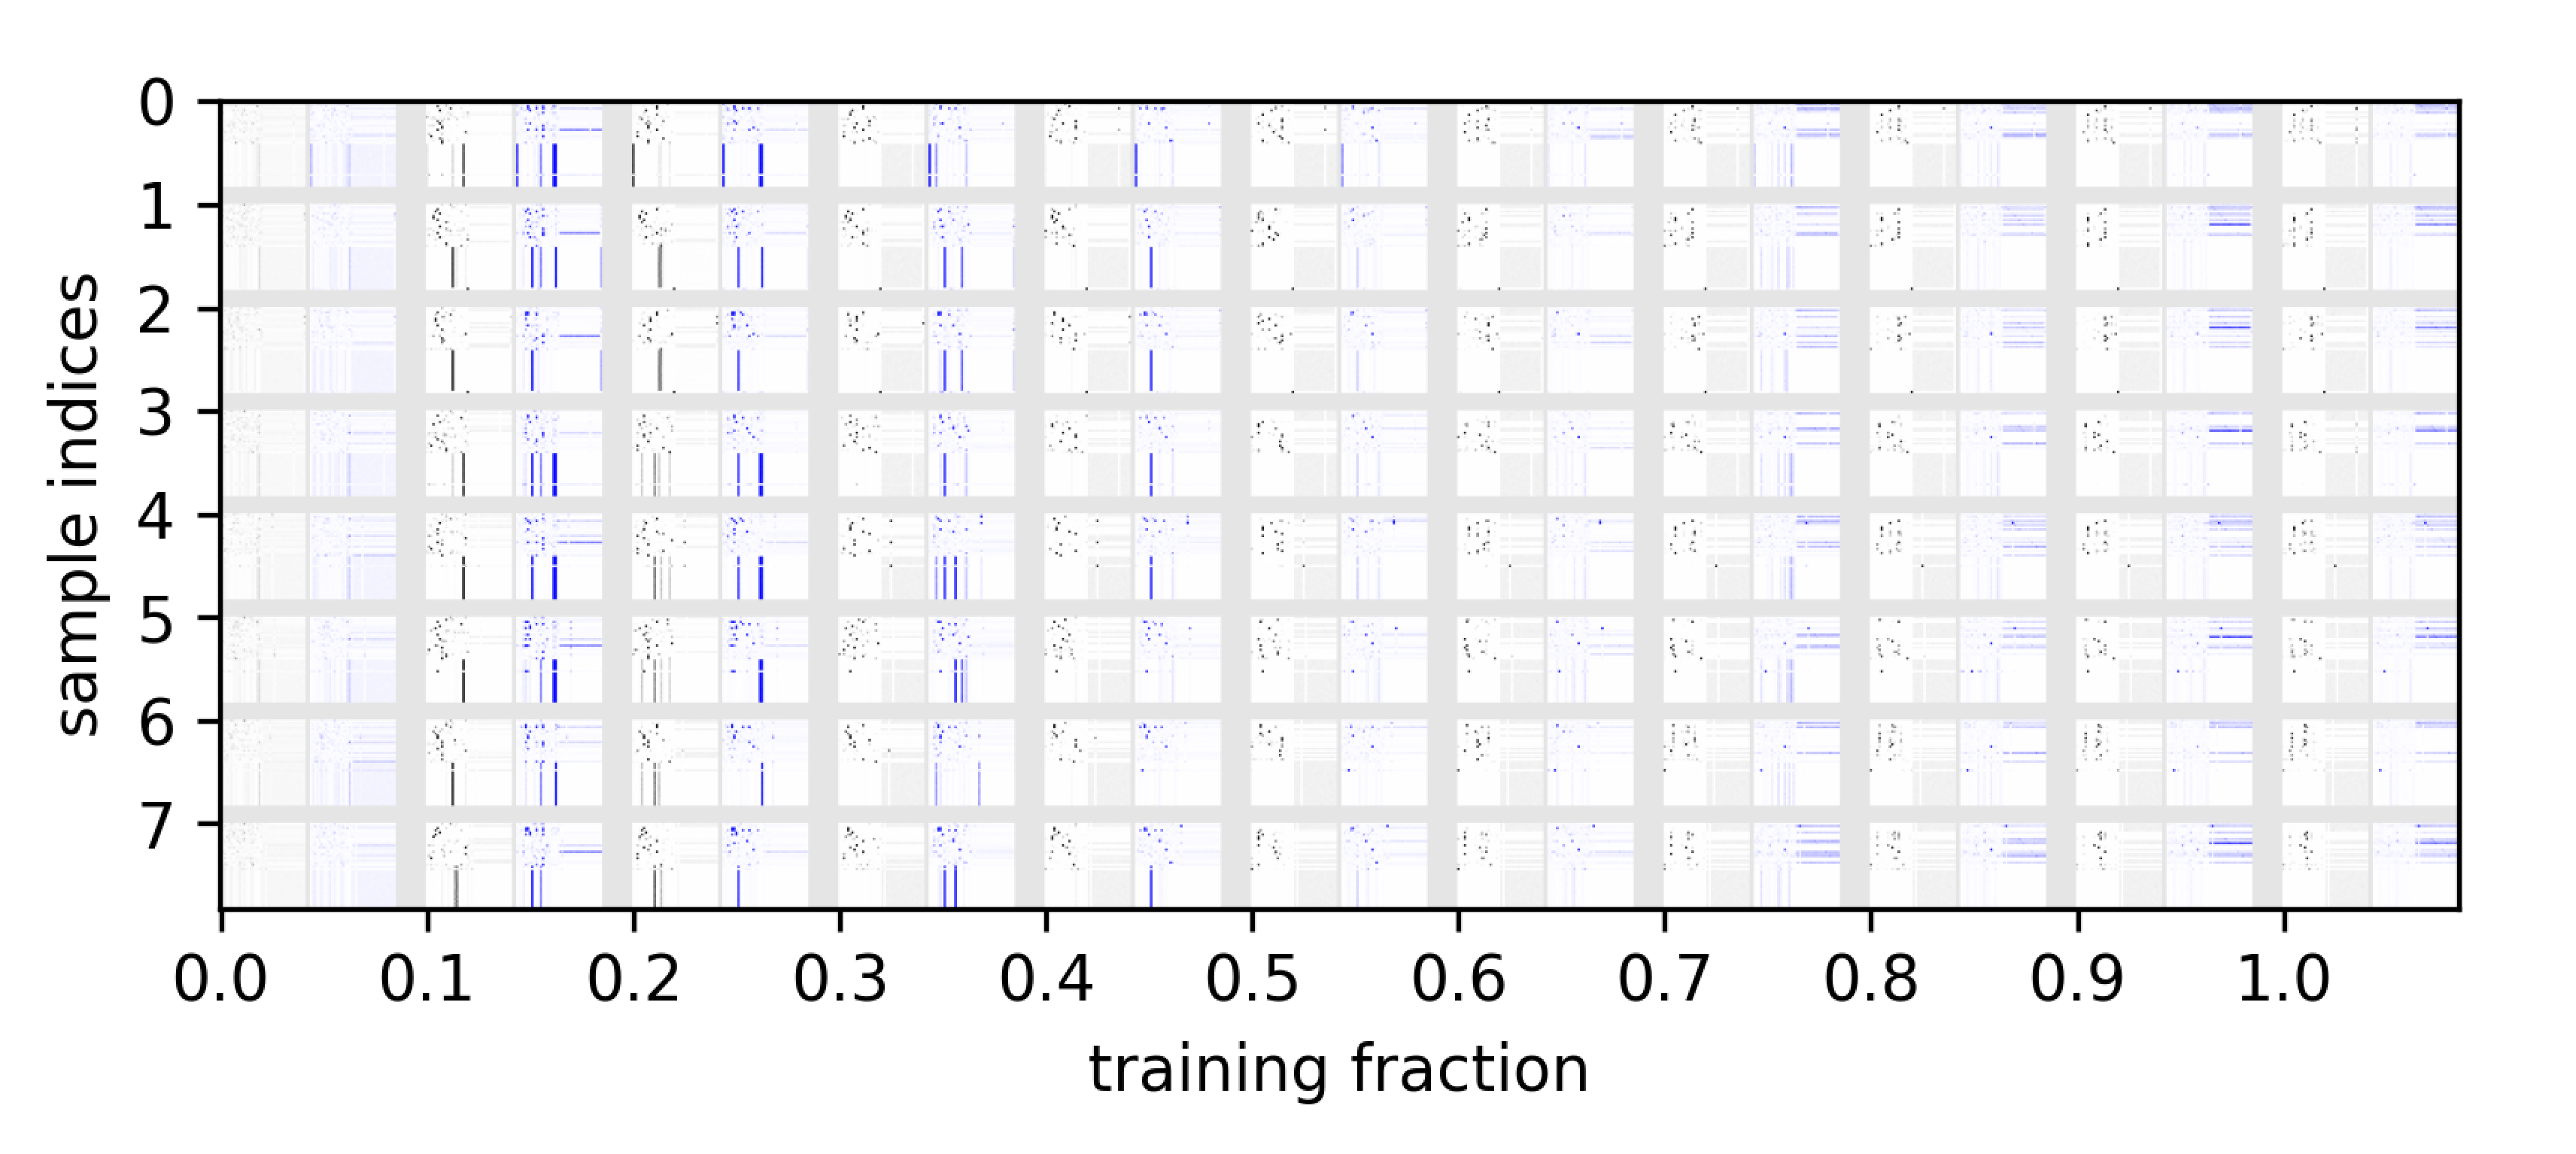
\includegraphics[width=\textwidth]{figures/attn_progress_by_sample_large2.png}
    \caption{For 8 samples, the post-activation attentions is visualized as training progresses on the $k=1, n=40$ summation problem.  The model has one head to simplify the visualization.  The attention is shown in pairs for each sample with softmax attention is in black and sigmoid is in blue.  A $2 \times 2$ block structure is evident in both cases, resulting from each halve of the input containing different information.}
    \label{fig:attn_by_sample}
\end{figure}



\subsubsection{Pair Repeat Problem}
\label{sec:a_se_pair_repeat_prob}

We define a synthetic task of identifying if the first two symbols in a sequence repeat.  The symbols, $s_i$ below come from a fixed vocabulary of size $K$, and the repeat location (when present) is uniformly distributed in the sequence.

\begin{center}
\begin{math}
f(s_0, s_1, s_2, ..., s_N) = \begin{cases}
1, & \text{ if } \exists \ n>1 \mid (s_0, s_1) = (s_n, s_{n+1}), \\
0 & \text{ otherwise}
\end{cases}
\end{math}
\end{center}

A simple two layer transformer is trained on this problem.  The model has an embedding dimension of 160, MLP ratio of 4, QK norm, and layers with eight heads.  The results for different model architectures are shown in Figure \Cref{fig:repeat_seq_results}.  The maximum input length is 22, $K=9$, shorter lengths are padding with value $K$, and the training set only contains lengths 14 and 15.  A cosine learning rate schedule with 5\% linear warmup and a maximum learning rate of 1e-3 is used with the Adam optimizer.  

In this result, we see the sigmoid activation has higher data efficiency and similar fall-off in the out of distribution cases.  From shorter runs, we estimate that the softmax network would fit the training with 4--5x more data.  Our conjecture is that the two layer transformer more easily learns the pair finding task with sigmoid because softmax is biased to focus on single values, though it is unclear why multiple heads are not able to compensate for this proposed cause in the softmax case.

\begin{figure}[h]
    \centering
    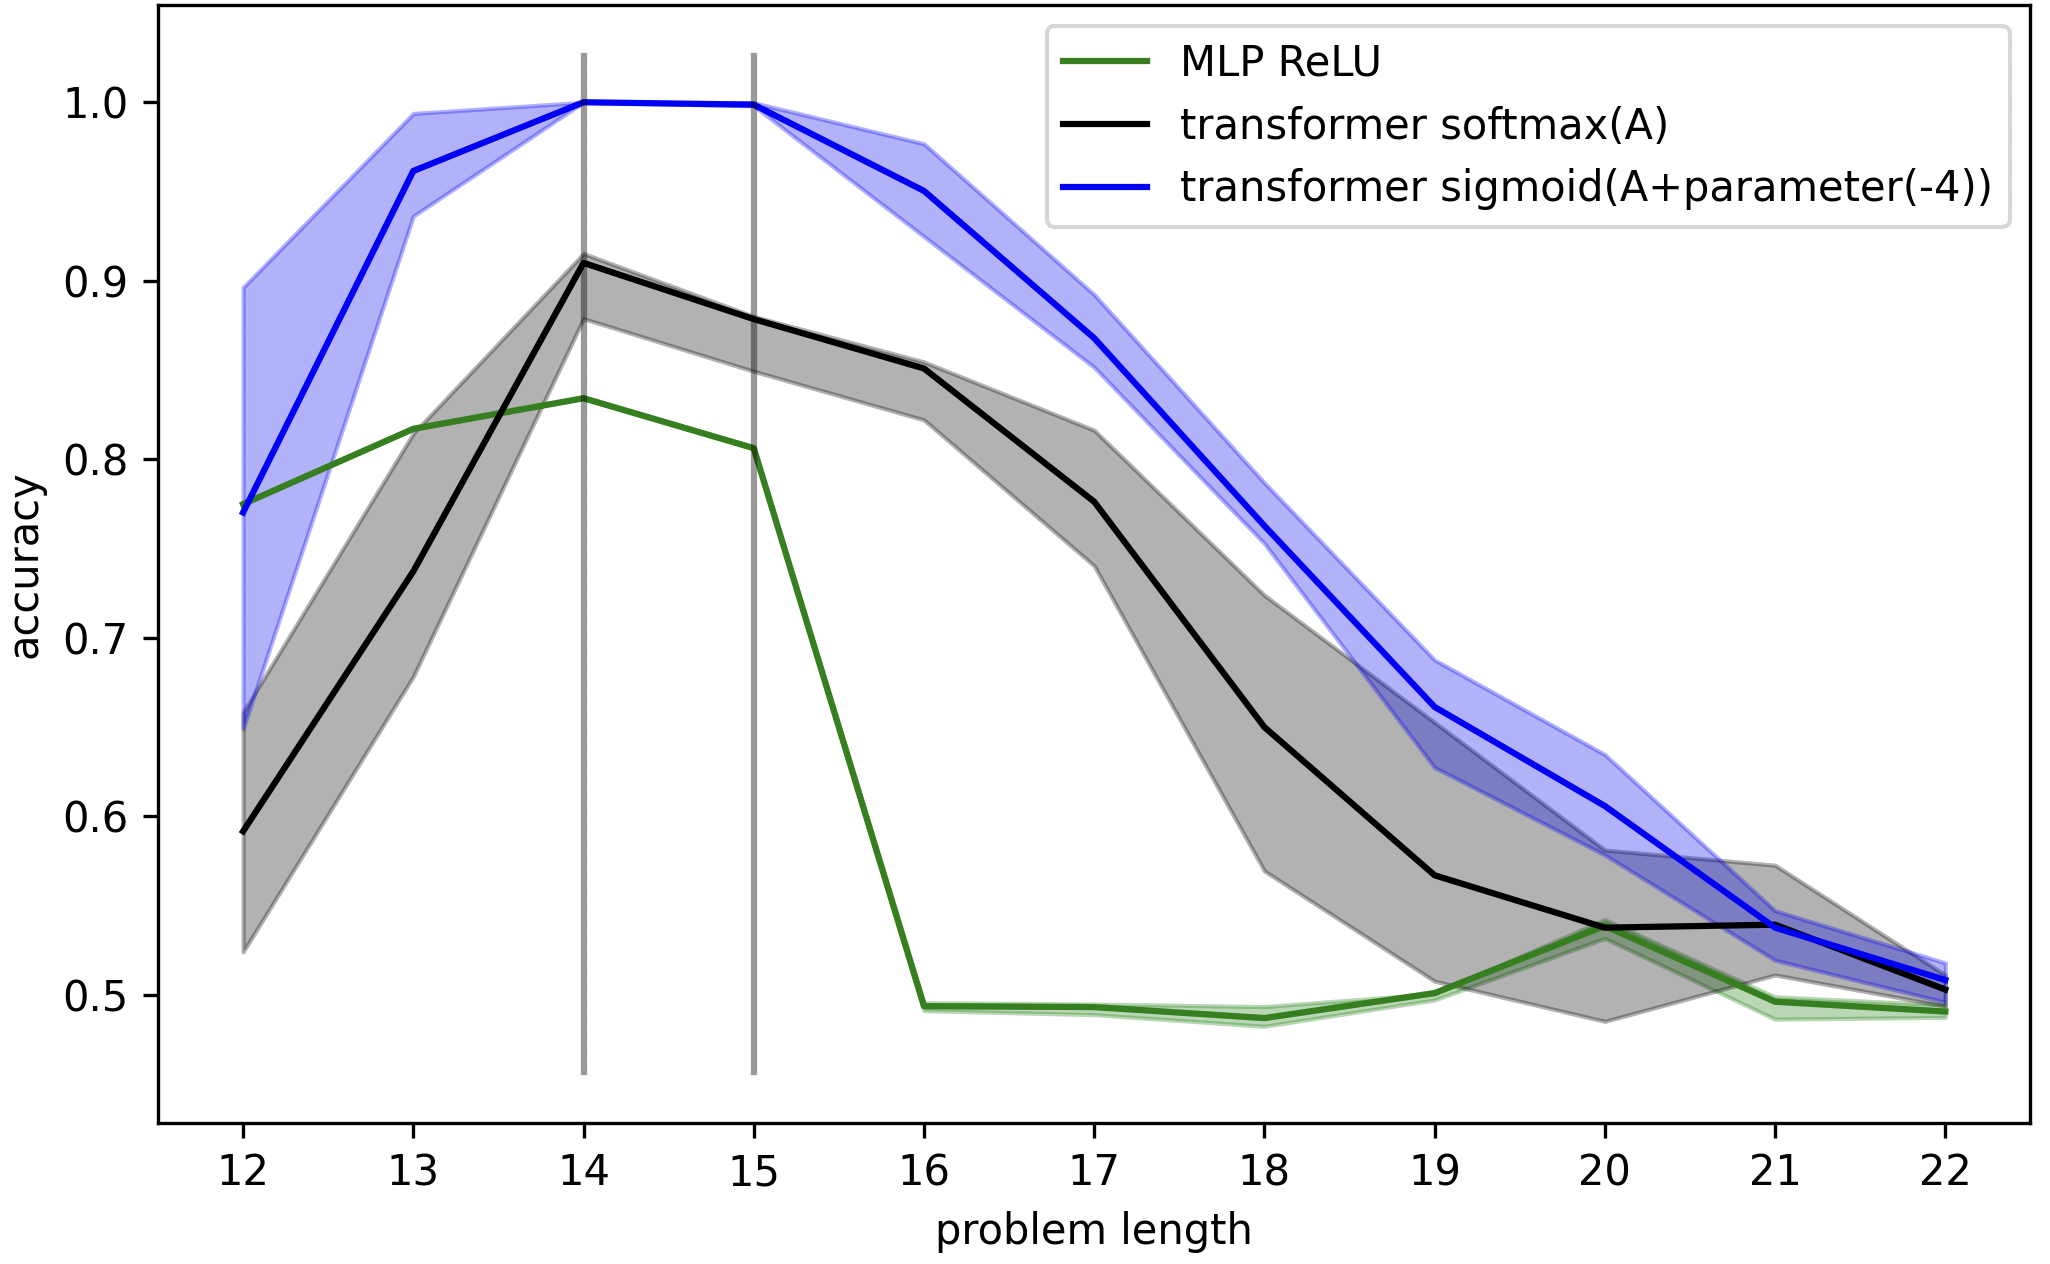
\includegraphics[width=0.7\textwidth]{figures/seq_length_results.png}
    \caption{Validation accuracy for out of distribution sequence lengths is shows after 5M samples of training; trained lengths are shown with vertical lines.  Quartiles and means are shown from six trials.  The MLP has two hidden layers, ReLU activation, and a similar number of parameters.  The sigmoid transformer has a learned offset initialized to -4.}
    \label{fig:repeat_seq_results}
\end{figure}
